\chapter{System Evaluation}\label{chap:Eval}
This section of the dissertation concerns evaluating the projects objectives set out in the introduction chapter \ref{chap:intro}, alongside the aforementioned, any limitations with the project, manual testing, and automated testing will also be discussed. 

\section{Cypress}
The system uses end to end testing \cite{E2ETesing} in the cypress automated testing environment, which tests the application under real time user experiences. The below are the specs which were created for the application.

\begin{figure}[h!]
    \centering
    \includegraphics[width=0.5\textwidth]{images/spec.png}
    \caption{Specs for testing the application}
    \label{image:spec}
\end{figure}

\section{Objectives}
The following are the project's objectives, which are listed in the introduction:

\begin{itemize}
    \item To create a dynamic single page application.
    \item The user can register their own account with the application.
    \item The user can sign into their own account once     	registered.
    \item A user is able to post pictures, they wish to share with their friends/family.
    \item Users can search for certain memories using taglines or memory titles.
    \item Users can send messages between each other.
    \item A user is allowed to like a picture, and comment underneath it.
    \item Users can create bio's underneath their posts.
    \item Users should be able to login to their profile and logout.
    \item Designing test scenarios to use in conjunction with cypress automated test tool. 
    \item To have a fully automated test features to verify    the application for commercial use, using test case scenarios designed.
\end{itemize}

The above will be analyzed below as to how well these objectives were completed.

\subsection{To create a dynamic single page application}
Manual testing revealed that the application is a single page application, only manual testing could be used at this level because it is difficult to determine unique ids that appear in urls such as the one below.
\begin{figure}[h!]
    \centering
    
\includegraphics[width=0.4\textwidth]{images/id.png}
    \caption{A dynamic id assigned to a post}
    \label{image:id}
\end{figure}
The key advantage of creating a single page application being the user does not have to re route multiple times to get to the page they wish to be on, also quicker loading times aiding the user experience \cite{jadhav2015single}.

\subsubsection{Other Examples of Dynamic Routing}
Other areas of the project where dynamic routing is used to make a single page application is through the below, the search bar, tags, and pagination.

\begin{figure}[ht]
\begin{minipage}[b]{0.5\linewidth}
    \centering
    
\includegraphics[width=\linewidth]{images/searchtag}
    \caption{Searching in use Dynamically}
    \label{image:searchtag}
\end{minipage}
    \hspace{0.5cm}
    \begin{minipage}[b]{0.3\linewidth}
    \centering
   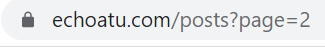
\includegraphics[width=\linewidth]{images/PaginationRoute}
    \caption{Paginate Dynamically through pages}
\end{minipage}
\end{figure}

\subsection{The user can register their own account with the application}
A user can manually create their own account by filling out the relevant form, or they can use Google's API for authorization. Manual and automated testing was recorded for manually signing up a user, but due to privacy restrictions, Google's API for signing up could only be tested manually.

\begin{figure}[h!]
    \centering
    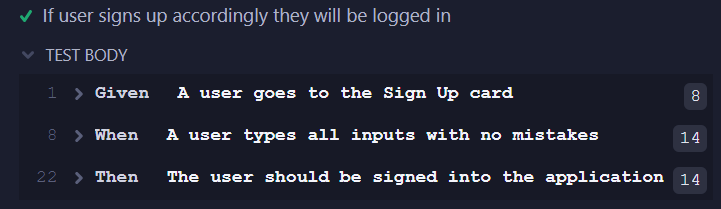
\includegraphics[width=0.4\textwidth]{images/TestPassSignUp.png}
    \caption{Specification for signing up a user manually passing}
    \label{image:TestPassSignUp}
\end{figure}

As shown above \ref{image:TestPassSignUp}, cypress is used to assert that when a user fills out the relevant fields in the authorization form, that user will be able to sign into the application, and thus a user can register to the application achieving this goal. Google's API is known to pass, but the user must have a Google account in order to use the aforementioned API, so automated testing would be ineffective. After completing this aim, testing discovered that not only was the original goal met, but it was also expanded to include two ways for a user to register with the application.

\subsubsection{Email Confirmation of sign in}
As an addition to signing up with the application, a user will be notified following successful sign up with a welcome message from the admin email. Testing of this feature was only conducted manually, setting up a mock email, after which checking their emails to see if the sendEmail api was called, which sends an email from the admin email address following sign up. The aforementioned test was successful, automating this case would not be possible due to security issues.

\subsection{The user can sign into their own account once registered}
The preceding section discusses signing up for the application, similarly signing into the application can be accomplished by using Google's API or manually entering information into the sign in form.

\begin{figure}[ht]
\begin{minipage}[b]{0.5\linewidth}
    \centering
    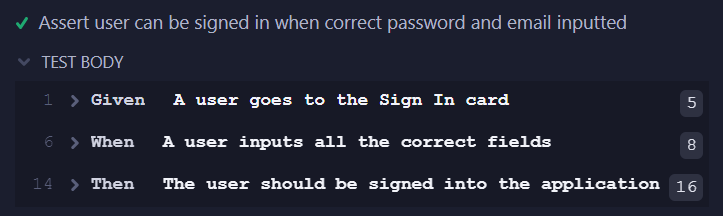
\includegraphics[width=\linewidth]{images/signinPass}
    \caption{Specification for signing in a user manually passing}
\end{minipage}
    \hspace{0.5cm}
    \begin{minipage}[b]{0.3\linewidth}
    \centering
   
\includegraphics[width=\linewidth]{images/SignedIn}
    \caption{User then signed in}
\end{minipage}
\end{figure}

Manual and automated testing has shown, that the user is able to sign into their account once it is created. Manual testing was preformed on Googles API, and on the sign in form. Automated testing was only preformed on the sign in form, not on Googles API. This objective similar to the above was also expanded upon to included Googles API for multiple ways to sign in to the application.

\subsection{A user is be able to post pictures, they wish to share with their friends/family}
If the authorization conditions are met, the user should be able to create a post and share it with all application users. In the terms of this objective, the user may also post a picture they wish to share, though this is optional, as the user may prefer not to share a picture and instead express their thoughts on current events.

\begin{figure}[ht]
\begin{minipage}[b]{0.4\linewidth}
    \centering
    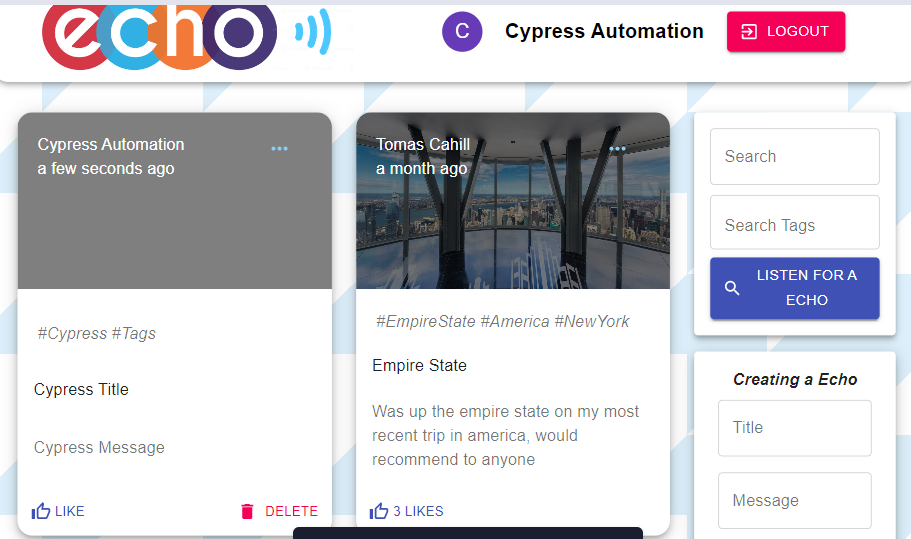
\includegraphics[width=\linewidth]{images/CreatedPost}
    \caption{Visual representation of created post}
    \label{image:CreatedPost}
\end{minipage}
    \hspace{0.5cm}
    \begin{minipage}[b]{0.4\linewidth}
    \centering
   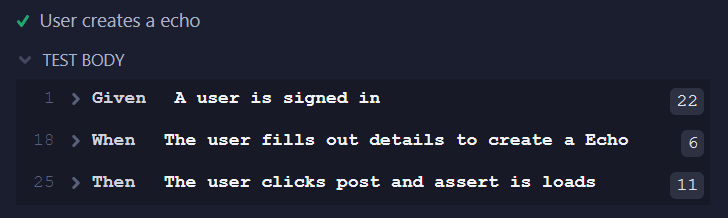
\includegraphics[width=\linewidth]{images/CreatedPostSpec}
    \caption{Automated test for user creating a post}
    \label{image:CreatedPostSpec}
\end{minipage}
\end{figure}

From the above figure \ref{image:CreatedPost}, it is shown the automated snapshot of running the specification from this figure \ref{image:CreatedPostSpec}. Due to limitations with the cypress testing tool, a picture could not be added to the post, however through manual behaviour testing preformed, it was found that a picture could be added when a file was chosen at the bottom of the creating a echo \ref{image:Form}.

\subsection{Users can search for certain memories using taglines or memory titles}
Searching in the application has been shown to be done in two ways as the requirements laid out, searching for a particular title, which is shown in this figure using a dynamic search system \ref{image:searchtag}. Moreover searching can be preformed through the use of tags \ref{image:SearchTags}.

\subsubsection{Search Testing using Title}
Carrying out automated testing on the search bar using the title of a post consisted of, inputting into the search bar what a user might search and then asserting that the right posts displayed on the screen, of which this test was found to be successful both manually and automated using cypress as can be seen below.

\begin{figure}[ht]
    \hspace{0.5cm}
    \begin{minipage}[b]{0.3\linewidth}
    \centering
   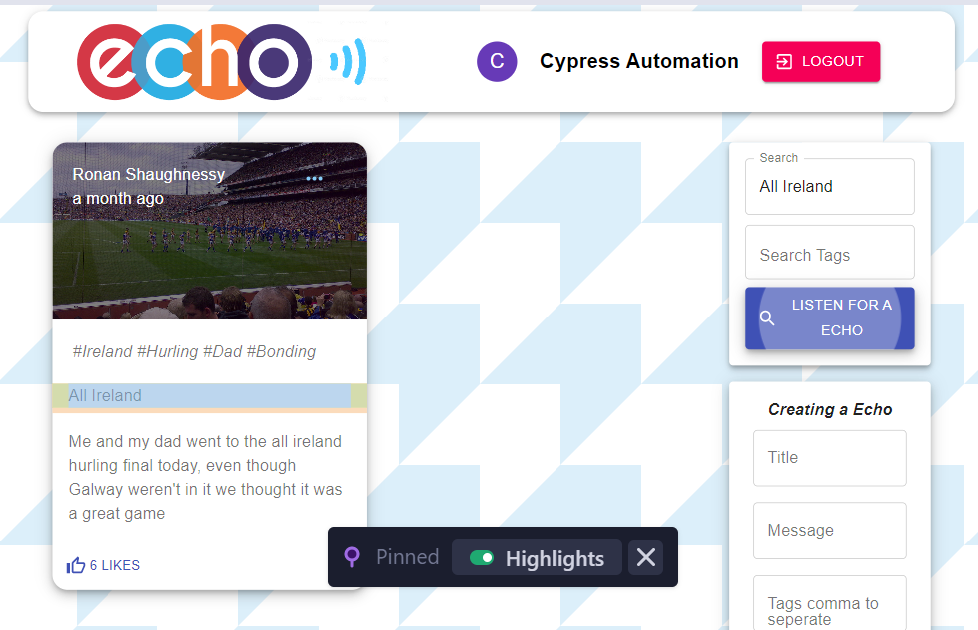
\includegraphics[width=\linewidth]{images/SearchTestSignedIn}
    \caption{Search bar test}
    \label{image:SearchTestSignedIn}
\end{minipage}
    \hspace{0.5cm}
    \begin{minipage}[b]{0.5\linewidth}
    \centering
   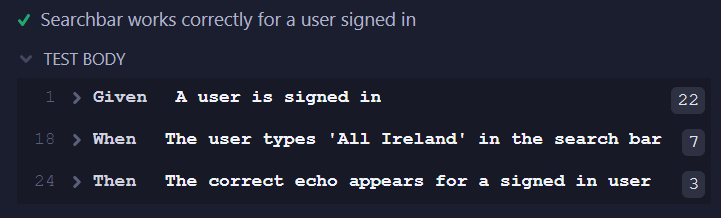
\includegraphics[width=\linewidth]{images/SignedInSeach}
    \caption{Using search bar test case}
    \label{image:SignedInSeach}
\end{minipage}
\end{figure}

\subsubsection{Search Testing using Tags}
Manual and automated testing was also preformed on tagline searches, of which searching using tags manually can be seen here \ref{image:SearchTags}. The automated version of testing can be seen below both types of testing were successful, although an element of flakiness can be seen in an automated test using tagline, which was found be attributed to the page being dynamically loaded.
\begin{figure}[ht]
    \hspace{0.5cm}
    \begin{minipage}[b]{0.3\linewidth}
    \centering
   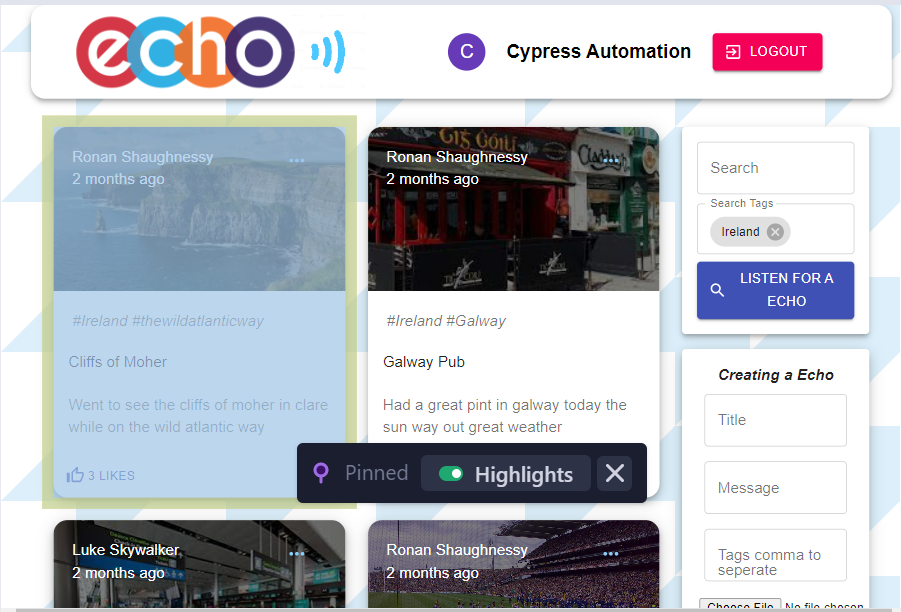
\includegraphics[width=\linewidth]{images/TagS}
    \caption{Asserting tagline working}
    \label{image:TagS}
\end{minipage}
    \hspace{0.5cm}
    \begin{minipage}[b]{0.5\linewidth}
    \centering
   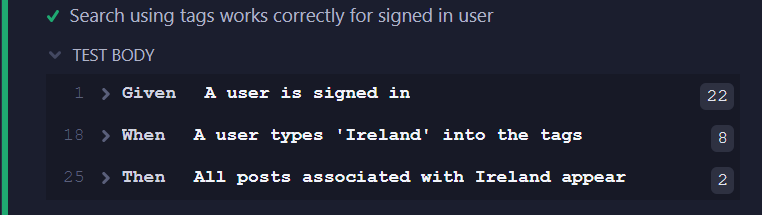
\includegraphics[width=\linewidth]{images/TagG}
    \caption{Tagline search test case}
    \label{image:TagG}
\end{minipage}
\end{figure}

\subsubsection{Search Testing using Tags and Title}
When the searching feature of the application was used to search for a title, and tags, an assertion had to be made to ensure both related posts appeared for the user. This was evaluated through the use of manual, and automated testing. Manual testing revealed that this feature was complete, and that the associated posts appears when the title and tagline inputs were filled. Automated testing was also conducted, and the results of the automated test can be seen below.
\begin{figure}[ht]
    \hspace{0.5cm}
    \begin{minipage}[b]{0.3\linewidth}
    \centering
   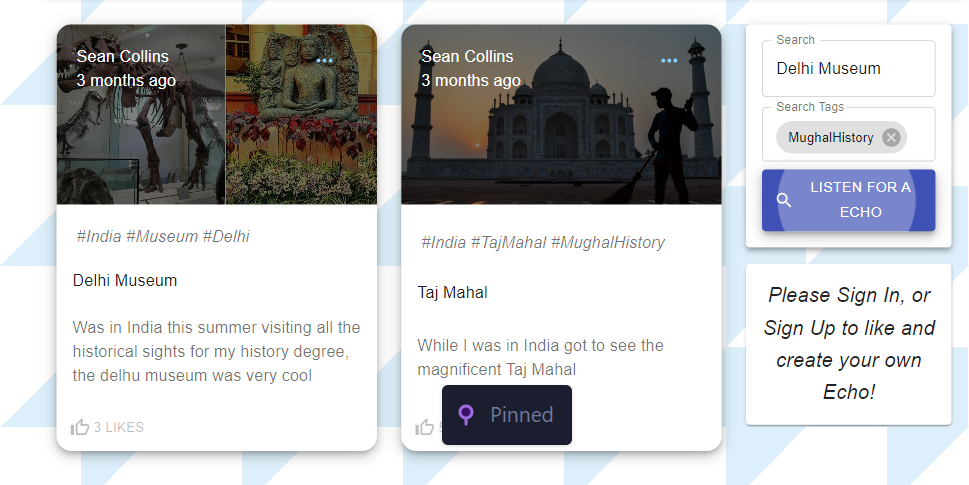
\includegraphics[width=\linewidth]{images/TagAndTitleSearch}
    \caption{Asserting tags and search title working together}
    \label{image:TagAndTitleSearch}
\end{minipage}
    \hspace{0.5cm}
    \begin{minipage}[b]{0.5\linewidth}
    \centering
   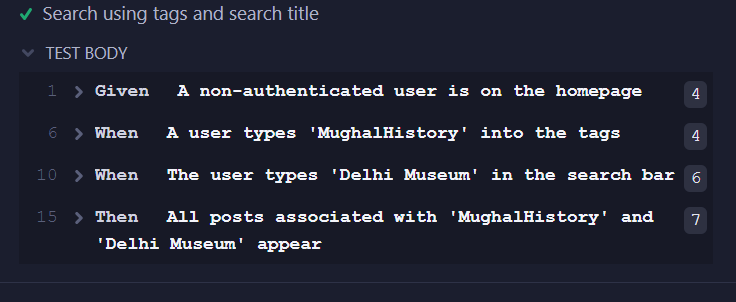
\includegraphics[width=\linewidth]{images/TagAndTitleSearchTestCase}
    \caption{Tags and search title test case}
    \label{image:TagAndTitleSearchTestCase}
\end{minipage}
\end{figure}

\subsection{Users can send messages between each other}
This objective of the project was not reached therefore, this aim is a failed component of the application. Due to time constraints this is why this part of the system was not implemented however, future iterations of the application may include messaging between users.

\subsection{A user is allowed to like a picture, and comment underneath it}
This objective passed, and has seen extensive testing, both automated and manually. This objective assumes the user is signed into the application.

\subsubsection{Liking a post}
Cypress has shown through the use of behaviour test development, that a user can like a post. In the below figure it is shown using a snapshot Cypress has taken of the application. As a result of the user clicking the like button, Cypress asserts that the application has updated the text to say "You and " then the number of likes present on the post previously, the text "You and " will only appear once a user has clicked like if they have not done so already . Manual testing was conducted prior to automated testing to ensure that the application dynamically updates to say "You and", to assert that the signed in user has liked the post.

\begin{figure}[ht]
\begin{minipage}[b]{0.4\linewidth}
    \centering
    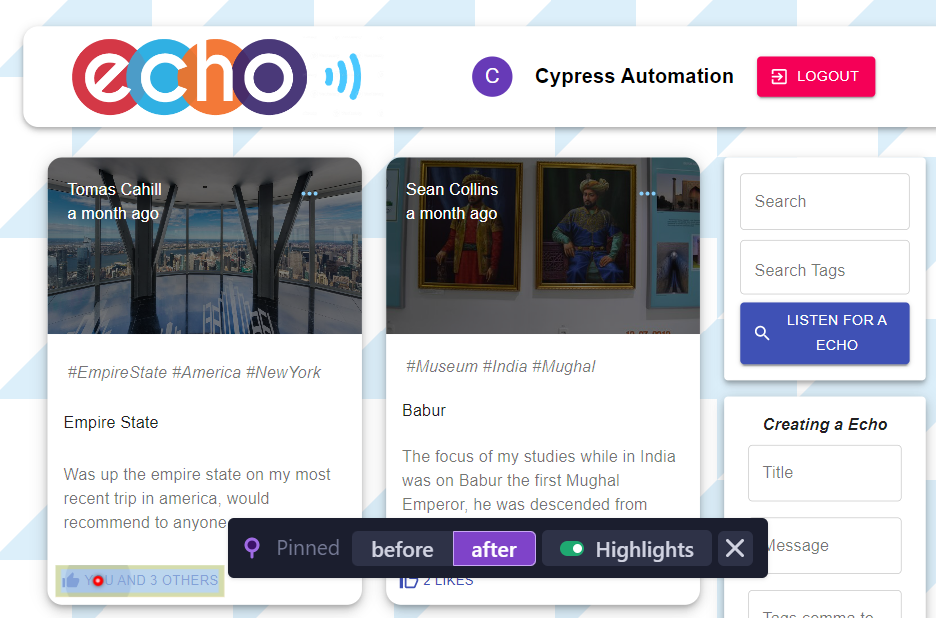
\includegraphics[width=\linewidth]{images/LikingSignIn}
    \caption{Liking a post when signed in}
    \label{image:LikingSignIn}
\end{minipage}
    \hspace{0.5cm}
    \begin{minipage}[b]{0.4\linewidth}
    \centering
   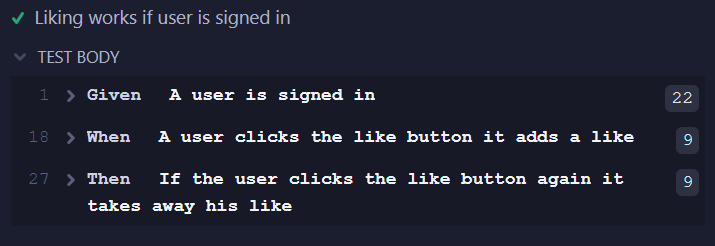
\includegraphics[width=\linewidth]{images/LikingFeature}
    \caption{Test case for liking}
    \label{image:LikingFeature}
\end{minipage}
\end{figure}

\subsubsection{Unliking a post}
Succeeding the above test, Cypress continues to follow user behaviour as seen in this figure \ref{image:LikingFeature}, by disliking the post after liking said post. This assertion checks that when a user clicks like again, the post will then revert to its previous from e.g 3 LIKES as shown below, and will no longer have the test "You and ".

\begin{figure}[h!]
    \centering
    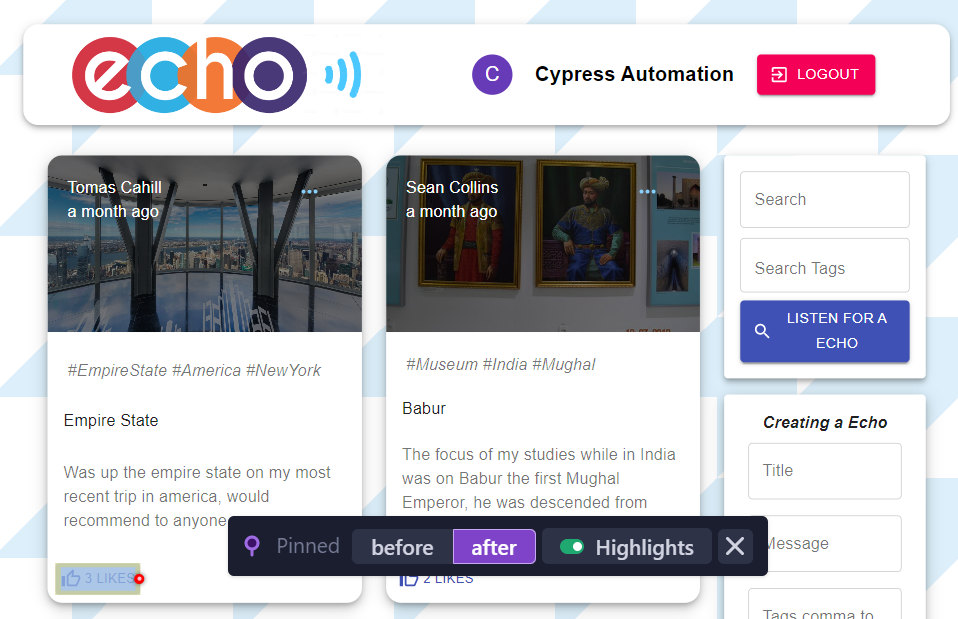
\includegraphics[width=0.5\textwidth]{images/Unliking.png}
    \caption{Unliking a post}
    \label{image:Unliking}
\end{figure}

\newpage
\subsubsection{Testing Comments Manually}
The user is able to comment in a post provided they are signed in. Testing was carried out manually by clicking the ellipses in the top right, which brings the user to the details of the post, of which this post screen can be seen from this figure \ref{image:PageDetails}. After which to carry out the test the comment box was clicked and a comment was inputted then the comment button was clicked, following this the comment appeared on the post thereby achieving this objective.

\subsubsection{Testing Comments using Cypress}
Cypress was employed to automatically simulate this behaviour, therein asserting that the test case passed automatically and that the objective that a user can comment on a post was met. The pretense was to type the content in the comment input box, click comment, and then assert that the username displays on the left under the comments area next to the comment which the user made.

\begin{figure}[ht]
\begin{minipage}[b]{0.4\linewidth}
    \centering
    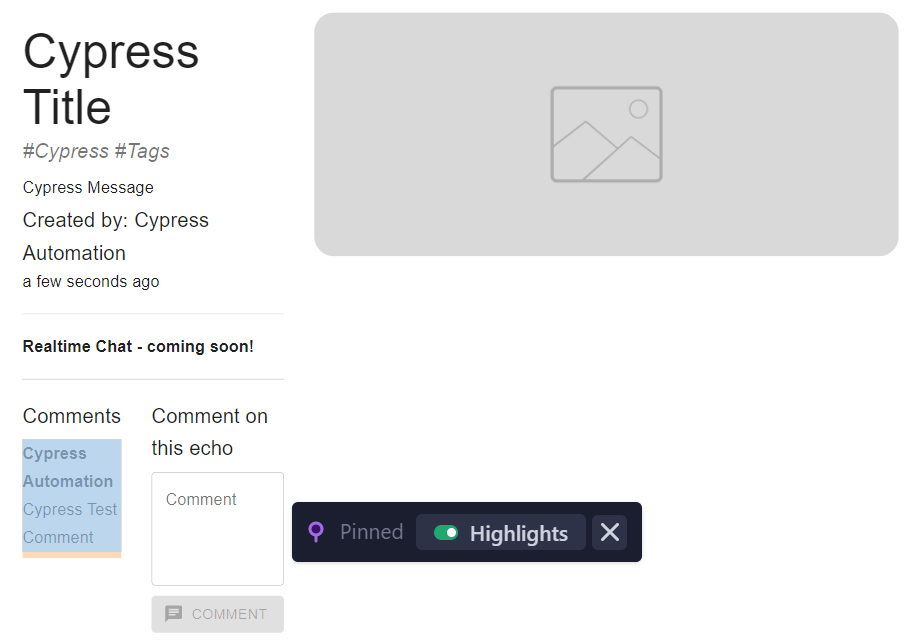
\includegraphics[width=\linewidth]{images/CommentTest}
    \caption{Cypress automating a comment}
    \label{image:CommentTest}
\end{minipage}
    \hspace{0.5cm}
    \begin{minipage}[b]{0.4\linewidth}
    \centering
   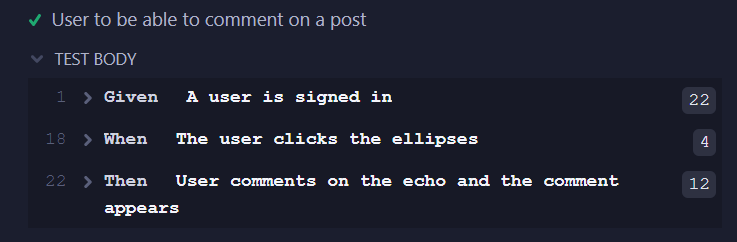
\includegraphics[width=\linewidth]{images/CommentTestCase}
    \caption{Test case for commenting on a post}
    \label{image:CommentTestCase}
\end{minipage}
\end{figure}

\subsection{Users can create bio's underneath their posts}
Users can when creating their post as seen in this figure \ref{image:Form}, make a bio or message to go with their post. While this objective has a limitation in that when the user is writing their message or bio, the message input box does not expand with the number of words the user is using, instead the input box remains the same length and width.

\subsubsection{Bio Testing}
Testing was conducted manually and automatically, only through manual testing was the above limitation found. However as seen below in cypress the user can create a bio under their post then create the aforementioned post.

\begin{figure}[h!]
    \centering
    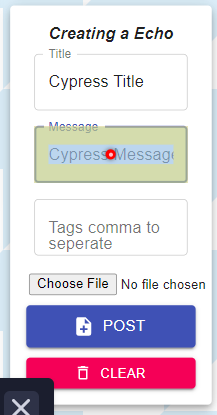
\includegraphics[width=0.3\textwidth]{images/MessageAuto.png}
    \caption{Cypress automatically creating a bio}
    \label{image:MessageAuto}
\end{figure}

\subsection{Users should be able to login to their profile and logout}
This objective tests the authorization of the application by asserting that a user can sign into the application, thereafter signing out if they wish.

\begin{figure}[h!]
    \centering
    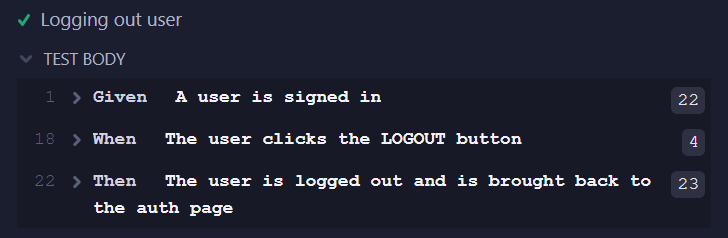
\includegraphics[width=0.5\textwidth]{images/LogInandOut.png}
    \caption{Test Feature for the above objective}
    \label{image:LogInandOut}
\end{figure}

\subsubsection{Logging into a profile}
Assertions were made to test the functionality of logging in manually and automatically. First manually testing, which was done by entering in the correct inputs, then asserting that the correct user was then signed into the application, which was found to have passed as the username appears in the navbar after signing in \ref{image:CyLogIn}. Secondly the automation suite asserted that a user could be signed in, Cypress did this by asserting the correct DOM element for a username appears on screen as shown below.

\begin{figure}[h!]
    \centering
    
\includegraphics[width=0.5\textwidth]{images/CyLogIn.png}
    \caption{Cypress asserting a user can log into their profile}
    \label{image:CyLogIn}
\end{figure}

\subsubsection{Logging out of a profile}
The last two steps from the feature above are done to assert that a user can log out of their profile, thereby completing this objective \ref{image:LogInandOut}. Firstly manual testing was preformed after coding was done, the finding was the logout button works, the user could log out of the application after they have signed in and have clicked the logout button. Finally, Cypress was used to take control of this test feature, automatically simulating the user's behavior. It was found to have passed as when Cypress clicks logout, the user is signed out and returned to the sign in form.

\begin{figure}[ht]
\begin{minipage}[b]{0.4\linewidth}
    \centering
    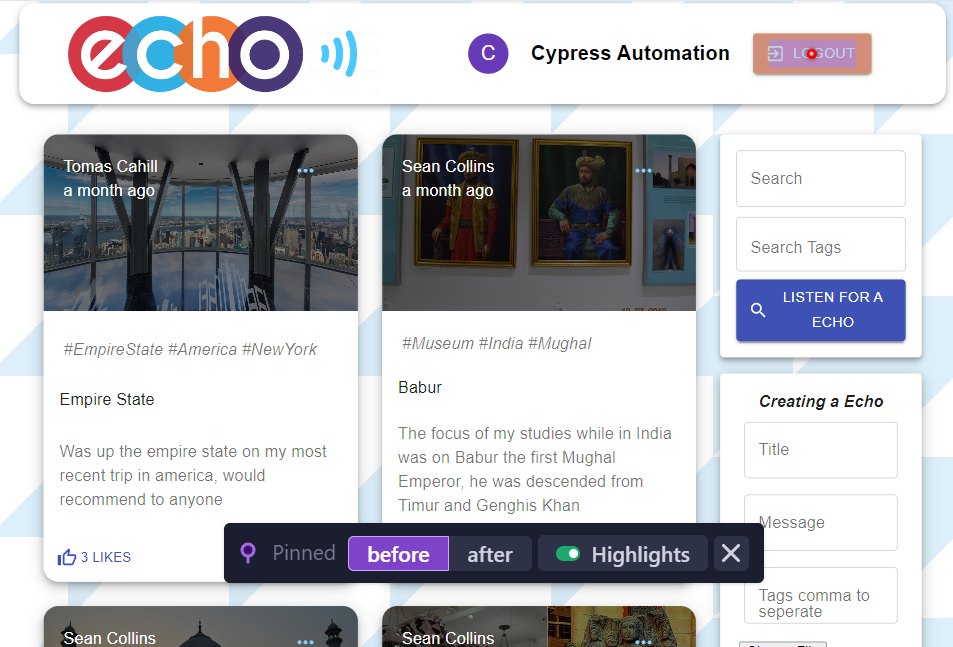
\includegraphics[width=\linewidth]{images/LogOutOne}
    \caption{Simulating clicking logging out}
    \label{image:LogOutOne}
\end{minipage}
    \hspace{0.5cm}
    \begin{minipage}[b]{0.4\linewidth}
    \centering
   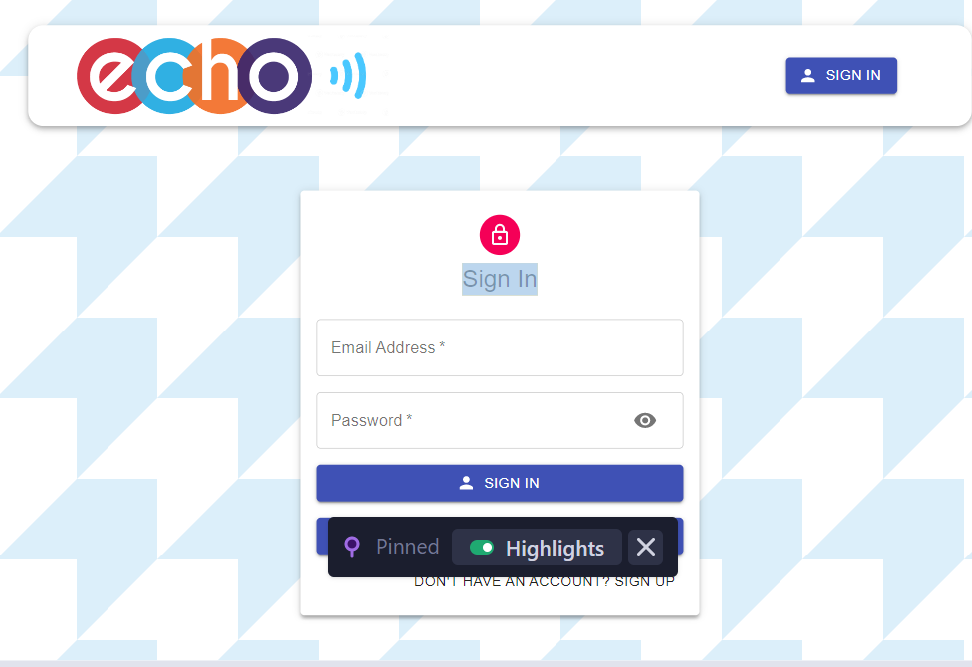
\includegraphics[width=\linewidth]{images/LogOutTwo}
    \caption{After click assert sign in form appears}
    \label{image:LogOutTwo}
\end{minipage}
\end{figure}

\newpage
\subsection{Designing test scenarios to use in conjunction with cypress automated test tool}
To achieve this goal, research was conducted in order to verify the best way of implementing appropriate language for use in the test scenarios. To that end gherkin syntax was employed, in order for anyone to understand the test cases that were to be written, see this section on gherkin syntax, and how it can be used to work with cypress \ref{sec:cypress-cucumber}. Numerous test scenarios was created for the application, some of which can be seen in the above sections of this chapter, the core concept for designing these test scenarios is that anyone could understand what the test is doing, even those who do not have a software development background. These referrals are the gherkin syntax in visual studio code, \ref{image:StepDefination} the first reference is the logic code which is used to assert the authentication system works appropriately, \ref{image:Feature} the second is the plain English employed in the steps for a given scenario, the last reference is to how the gherkin format looks when it is being executed through the cypress environment \ref{image:LogInandOut}. A full list of all test scenarios can be found on GitHub \href{https://github.com/Rshocks/Final-Year-Project/tree/main/QAautomation/cypress/e2e/features}here.

\subsection{To have a fully automated test features to verify the application for commercial use, using test case scenarios designed}
Employing the above objective to support this aim, using gherkin syntax in cypress in order to format the test scenarios. Following completion of the above goal, TypeScript was used to develop the test assertions, e.g. assert that a users name appears when a user is signed in, this maintains that a user name will appear once a user is signed in, asserting the appropriate user is logged into the application. This objective was therein achieved, as the application has a fully automated test suite, allowing for changes to be made in the development of the application, then the automated tests can run against the changes made in development, in order to assert changes to the code base has not altered any other feature of the application. The below table is a result of the automated tests carried out on the application, a flaky test is a test which passes sometimes, then fails other times.

\begin{table}
\centering
    \begin{tabular}{|c|p{3cm}|c|c|c|}
    \hline
    \multicolumn{5}{|c|}{Automated Testing Results} \\
    \hline
    Feature Name & Number of Test Cases & Pass & Failed & Flaky \\
    \hline
    \hline
        authForm & 9 & 6 & 0 & 3 \\
        pageDetails & 4 & 4 & 0 & 0 \\
        routes & 9 & 9 & 0 & 0 \\
        search & 7 & 6 & 0 & 2 \\
        userActions & 6 & 6 & 0 & 0 \\
    \hline
    \end{tabular}
\caption{Cypress Automated Testing Results}
\label{table:CyAutoResults}
\end{table}

\subsubsection{Flaky Tests}\label{Flaky}
Three flaky tests were observed in the authorization feature authForm. Two of which were asserting a pop up appears on screen when the user has not filled out a relevant part of the sign in or up form. While both these tests do pass technically, it can only be seen to pass visually when the programmer visually sees the pop up appear, as it was hard to be able to assert a pop up using cypress. Secondly a flaky test was seen in signing a user up, the user signs up correctly when the spec is run for the first time, however if the spec is re run, the scenario will fail as the user is already created, this prompts the admin of the database to manually delete the user for MongoDB.

\subsubsection{Solving Flaky Tests in the Future}\label{SolveFlaky}
Solving the pop up issue so the test does not have to rely the developer visually seeing the pop up, further code must be written and documentation studied on how to assert pop up boxes. Lastly, instead of the admin removing the user from the MongoDB database, there could be a way in cypress to use a different new email when the email is already in use thereby passing the test consistently, however this could crowd the database with null users if the spec is run often.

\section{Automation Results In Cypress}
The below are the visual results of the table above \ref{table:CyAutoResults}.
\begin{figure}
        \centering
        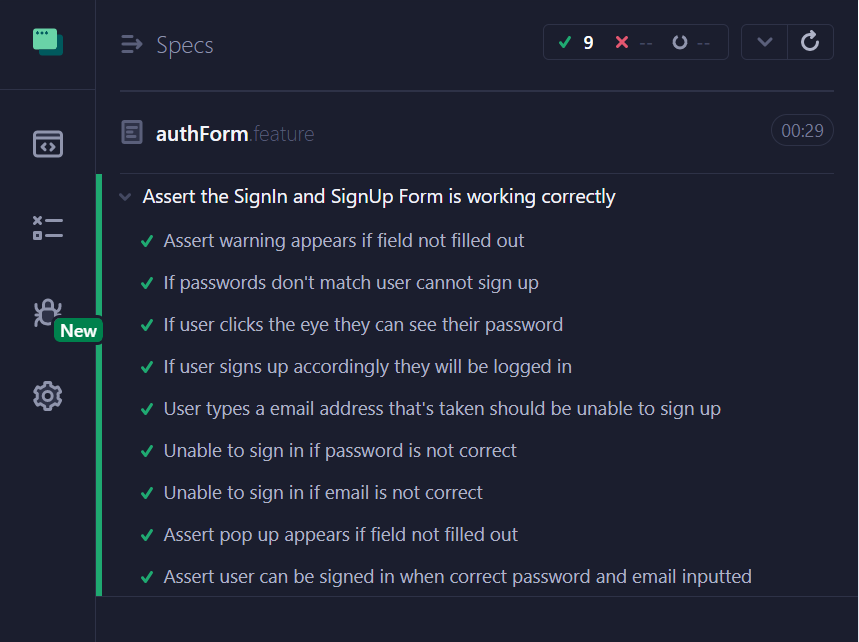
\includegraphics[width=0.28\textwidth]{images/authFormF}
        \hfill
        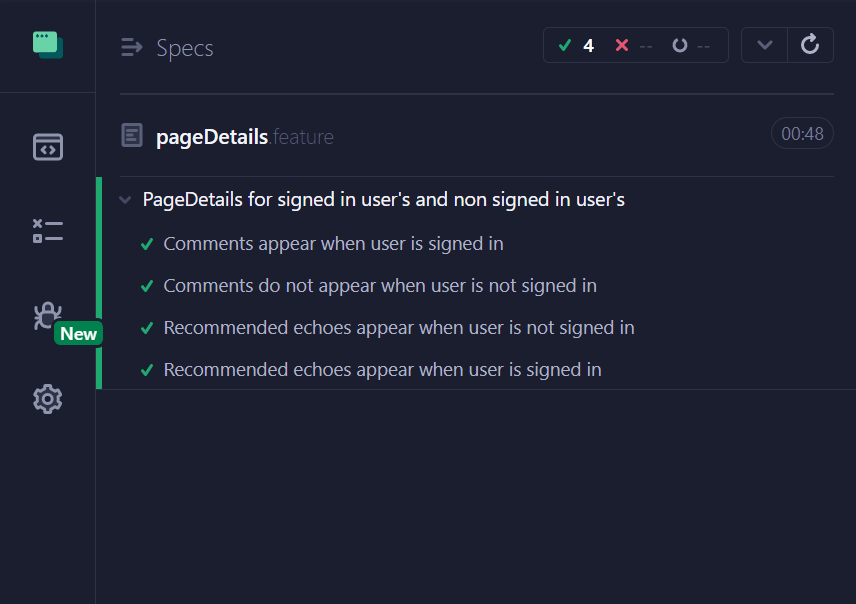
\includegraphics[width=0.28\textwidth]{images/pageDetailsF}
        \hfill
        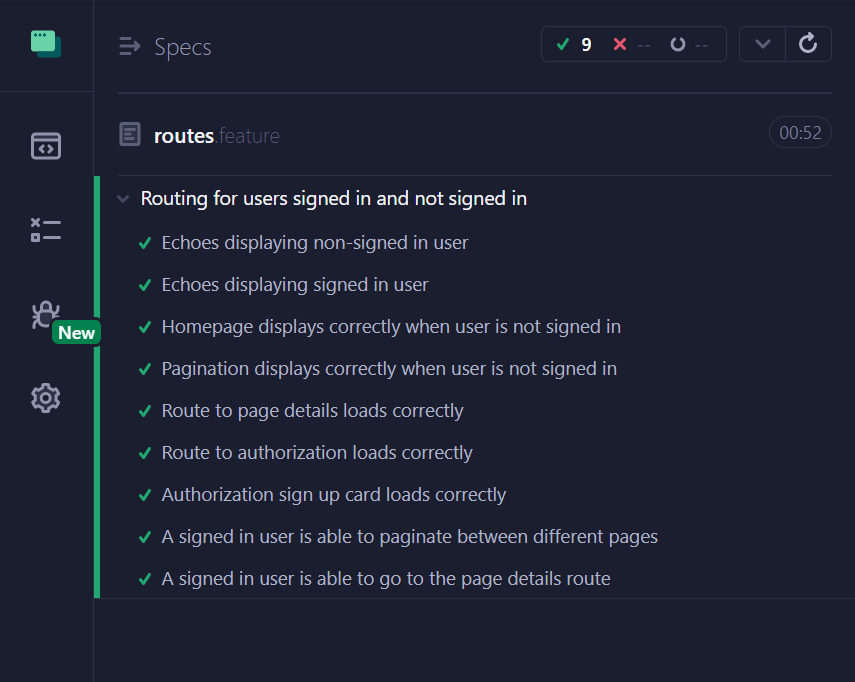
\includegraphics[width=0.28\textwidth]{images/RoutesF}
        \hfill
        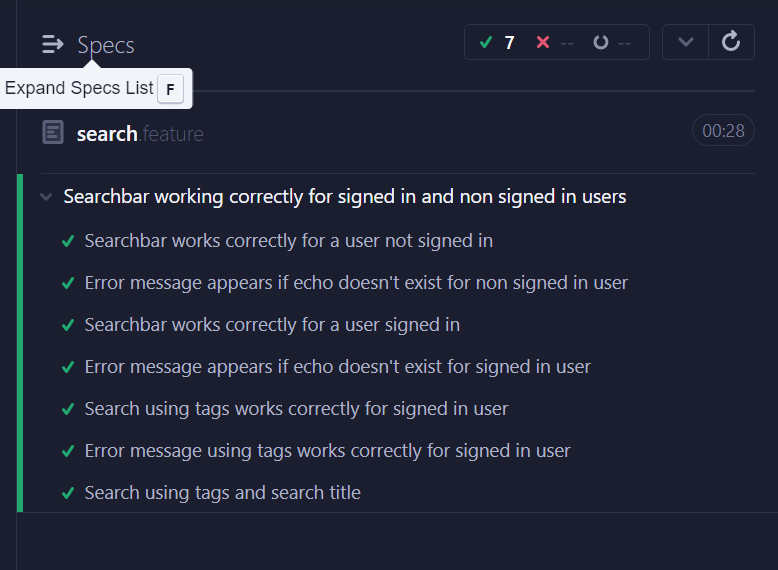
\includegraphics[width=0.28\textwidth]{images/SearchF}
        \hfill
        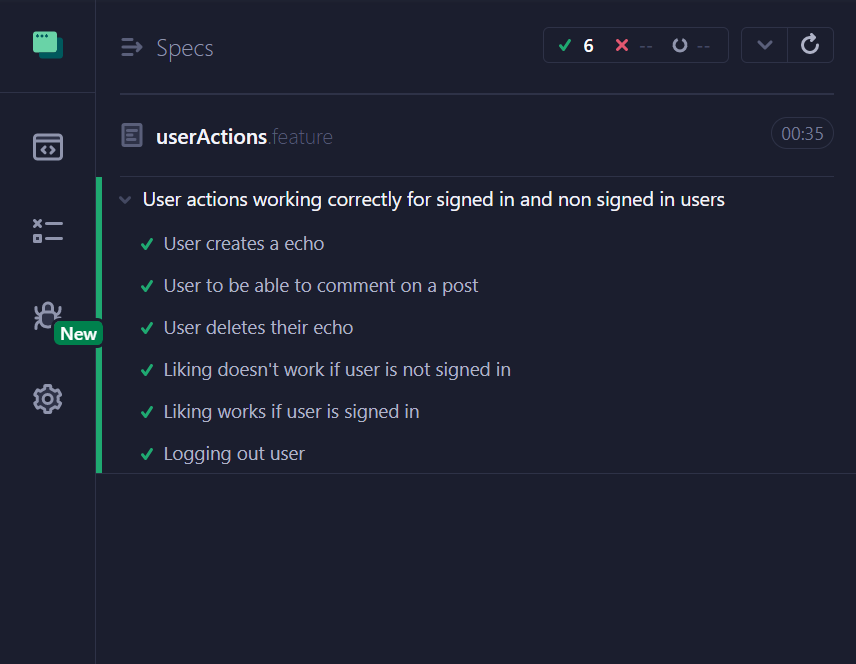
\includegraphics[width=0.28\textwidth]{images/UserActionsF}
        \caption{Five E2E Features}
\end{figure}

\section{Limitations}\label{sec:Limit}
While most objectives were met, creating a messaging system still eludes the application, perhaps in the future using front end technology a real time chat box will be implemented into the section donated for it in the page details component, this chat box would be linked into the page details, of who is active on a certain page detail e.g users on the New York page details post will be able to chat to other users, assuming they are present on the page at the same time, after which the conversation is over the application will automatically delete it. Other limitations include the section of flaky tests covered above \ref{Flaky}. Additional limitations noted while testing the application are, to automated a spike test on the application in order to ascertain how many users the application can handle, develop a forgotten password system when the user forgets their password, and deploying the system in the app store for phone users rather than having it in the browser on a mobile.